% %=====================================
% % Author: Christian Fischer Pedersen
% % About: Slide template
% %=====================================
%%==============================
%   Author: Christian Fischer Pedersen
%   About: Beamer style file
%==============================

%========General
\documentclass[compress,mathserif,presentation,notheorems]{beamer}
%\usepackage[export]{adjustbox}
\usepackage{etex}
\usepackage[utf8]{inputenc}%Danske bogstaver
\usetheme{default}
\usecolortheme{default}

%========Fonts
\setbeamercolor{structure}{fg=aaudblue}
\setbeamerfont{structure}{family=\sf\bfseries}
\setbeamercolor{normal text}{fg=black}
\setbeamerfont{normal text}{family=\sf\mdseries}
\renewcommand{\footnoterule}{}
\renewcommand{\footnotesize}{\tiny}

%========Sections
\AtBeginSection[]{\begin{frame}\frametitle{Outline}\tableofcontents[currentsection]\end{frame}}

%========Parts
\makeatletter
\AtBeginPart{%
  \addtocontents{toc}{\protect\beamer@partintoc{\the\c@part}{\beamer@partnameshort}{\the\c@page}}%
}
%% number, shortname, page.
\providecommand\beamer@partintoc[3]{%
  \ifnum\c@tocdepth=-1\relax
    % requesting onlyparts.
    \sf{\bf{\textcolor{aaudblue}{\makebox[6em]{PART #1:}#2}}}
    \par
  \fi
}
\define@key{beamertoc}{onlyparts}[]{%
  \c@tocdepth=-1\relax
}
\makeatother

%========Itemize and enumerate
\setbeamertemplate{itemize items}[triangle]%triangle,circle,ball,square
\setbeamertemplate{note page}[plain]

%========Colors
\usepackage{pstricks,pst-node}
\newrgbcolor{aaudblue}{0.2 0.4 0.6}   %dark blue
\newrgbcolor{aaulblue}{0.4 0.6 0.8}   %light blue
\newrgbcolor{lgray}   {0.9 0.9 0.9} %light gray
\definecolor{lgray}{rgb}{0.9,0.9,0.9} %light gray
\definecolor{mgray}{rgb}{0.5,0.5,0.5} %medium gray
\definecolor{dgray}{rgb}{0.2,0.2,0.2} %dark gray

%========Footer
\beamertemplatenavigationsymbolsempty
\usepackage{tabularx}
\setbeamertemplate{footline}{
%\colorbox{white}
{\color{aaudblue}
\begin{tabularx}{0.98\textwidth}{l X}
~\insertshortauthor, \insertshortinstitute & \hfill \insertframenumber$|$\inserttotalframenumber\\
\end{tabularx}
}\vskip6pt
}

%========Header
\setbeamercolor*{palette tertiary}{fg=aaudblue,bg=white}
\setbeamertemplate{headline}{%
\begin{beamercolorbox}{section in head/foot}
\vskip6pt \insertsectionnavigationhorizontal{\paperwidth}{}{} \vskip2pt
%\vskip6pt \insertnavigation{\paperwidth} \vskip2pt
\end{beamercolorbox}%
}

%========Title page
\newcommand{\slidetitlepage}[2]{
\title{#1}
\subtitle{#2}
\author[Christian Fischer Pedersen]%
{Christian Fischer Pedersen\\[-1.4mm]%
%{\scriptsize Associate Professor, PhD}\\[-1.4mm]%
{\scriptsize cfp@eng.au.dk}}
\institute[Electrical and Computer Engineering, Aarhus University]%
{Section of Electrical and Computer Engineering\\
Department of Engineering\\
Aarhus University}
\date{{\scriptsize Revised on \today}}
}


%========Math fonts 
\usepackage{amsmath}
\usepackage{bbm}
\usepackage{pifont}
\usepackage{wasysym}
\usepackage{amssymb}
\usepackage{amsbsy}


%========Blocks
\setbeamertemplate{blocks}[rounded][shadow=true]
\setbeamercolor{block title} {bg=aaulblue,fg=white}
\setbeamercolor{block body}{bg=white,fg=black}%fg=lgray}

%========Figures and graphics
\usepackage[dvips]{epsfig}
\usepackage[dvips]{graphicx}
\usepackage{subfigure}
\usepackage{caption}%Skal komme efter 'subfigure' for ogsaa at virke paa denne
\usepackage{fancybox}\cornersize{1}
\usepackage{tikz}


%========Video and sound
%\usepackage{multimedia}


%========Tables
%\usepackage{booktabs}
\usepackage{rotating}
\usepackage{multirow}


%========Referencing and citations
\usepackage[sort&compress, numbers]{natbib}
\newcommand{\citefont}[1]%
{\fontsize{5pt}{5pt}\selectfont#1\normalsize}

\newcommand{\scite}[1]%Formerly known as "slidecite"
{\fontsize{5pt}{5pt}\selectfont(\citeauthor{#1}, \citeyear{#1} [\citenum{#1}])\normalsize}

\newcommand{\sciten}[1]%Formerly known as "slidecitenormal"
{(\citeauthor{#1}, \citeyear{#1} [\citenum{#1}])}

\newcommand{\scitennp}[1]%Formerly known as "slidecitenormalnp" - np means no parantheses 
{\citeauthor{#1}, \citeyear{#1} [\citenum{#1}]}

\newcommand{\scitesub}[1]%Formerly known as "slidecitesubmitted"
{\fontsize{5pt}{5pt}\selectfont(\citet{#1})\normalsize}

\renewcommand{\bibsection}{\subsubsection*{\bibname}} %Avoid 'References' in header

\newcommand{\shref}[2]%
{\href{#1}{\textcolor{aaudblue}{\textbf{#2}}}}

%\bibpunct[:]{(}{)}{;}{a}{}{,}

%========Misc. defines
\newcommand{\nolinefrac}[2]{\genfrac{}{}{0pt}{}{#1}{#2}}
\def\simiid{\overset{\scriptsize{i.i.d.}}{\sim}}
\def\CSMfac{$\textrm{CSM}_{\textrm{fac}}~$}
\def\CSMfft{$\textrm{CSM}_{\textrm{fft}}~$}
\def\Matlab{Matlab$^\copyright~$}
\def\rhoot{\mbox{\large{$\varrho$}}}

%========Vectors and matrices
\def\lambdav{\boldsymbol{\lambda}}
\def\lambdam{\mathbf{\Lambda}}
%\newcommand{\tlv}[1]{\tilde{\lv}^{{\raisebox{-2pt}{\footnotesize $(#1)$}}}} 
\def\deltav{\boldsymbol{\delta}}
\def\deltam{\mathbf{\Delta}}

%========Listings
\usepackage{listings}
% \lstset{
% nputencoding=T1,
% language=Matlab,
% xleftmargin=8pt,
% tabsize=2,
% basicstyle=\small, print whole listing small
% keywordstyle=\color{black}\bfseries, 
% identifierstyle=, nothing happens
% commentstyle=\color{black}\itshape,
% stringstyle=\color{black}\ttfamily,
% showstringspaces=false,
% numbers=left,
% stepnumber=0,
% numbersep=4pt,
% morekeywords={display}
% }

%Theorem environments
%----------------------------------------------------------
\usepackage{amsthm}
\theoremstyle{remark}
%\theoremstyle{definition}
\newtheorem{theorem}{Theorem}
\newtheorem{acknowledgement}{Acknowledgement}
\newtheorem{algorithm}{Algorithm}
\newtheorem{axiom}{Axiom}
\newtheorem{case}{Case}
\newtheorem{claim}{Claim}
\newtheorem{conclusion}{Conclusion}
\newtheorem{condition}{Condition}
\newtheorem{conjecture}{Conjecture}
\newtheorem{corollary}{Corollary}
\newtheorem{criterion}{Criterion}
\newtheorem{definition}{Definition}
\newtheorem{example}{Example}
\newtheorem{exercise}{Exercise}
\newtheorem{lemma}{Lemma}
\newtheorem{notation}{Notation}
\newtheorem{problem}{Problem}
\newtheorem{proposition}{Proposition}
\newtheorem{remark}{Remark}
\newtheorem{solution}{Solution}
\newtheorem{summary}{Summary}
\newtheorem{property}{Property}
\newtheorem{equivalence}{Equivalence}
\newtheorem{expression}{Expression}
%==============================
%   Author: Christian Fischer Pedersen
%   About: Beamer style file
%==============================

%========General
\documentclass[compress,mathserif,presentation,notheorems]{beamer}
%\usepackage[export]{adjustbox}
\usepackage{etex}
\usepackage[utf8]{inputenc}%Danske bogstaver
\usetheme{default}
\usecolortheme{default}

%========Fonts
\setbeamercolor{structure}{fg=aaudblue}
\setbeamerfont{structure}{family=\sf\bfseries}
\setbeamercolor{normal text}{fg=black}
\setbeamerfont{normal text}{family=\sf\mdseries}
\renewcommand{\footnoterule}{}
\renewcommand{\footnotesize}{\tiny}

%========Sections
\AtBeginSection[]{\begin{frame}\frametitle{Outline}\tableofcontents[currentsection]\end{frame}}

%========Parts
\makeatletter
\AtBeginPart{%
  \addtocontents{toc}{\protect\beamer@partintoc{\the\c@part}{\beamer@partnameshort}{\the\c@page}}%
}
%% number, shortname, page.
\providecommand\beamer@partintoc[3]{%
  \ifnum\c@tocdepth=-1\relax
    % requesting onlyparts.
    \sf{\bf{\textcolor{aaudblue}{\makebox[6em]{PART #1:}#2}}}
    \par
  \fi
}
\define@key{beamertoc}{onlyparts}[]{%
  \c@tocdepth=-1\relax
}
\makeatother

%========Itemize and enumerate
\setbeamertemplate{itemize items}[triangle]%triangle,circle,ball,square
\setbeamertemplate{note page}[plain]

%========Colors
\usepackage{pstricks,pst-node}
\newrgbcolor{aaudblue}{0.2 0.4 0.6}   %dark blue
\newrgbcolor{aaulblue}{0.4 0.6 0.8}   %light blue
\newrgbcolor{lgray}   {0.9 0.9 0.9} %light gray
\definecolor{lgray}{rgb}{0.9,0.9,0.9} %light gray
\definecolor{mgray}{rgb}{0.5,0.5,0.5} %medium gray
\definecolor{dgray}{rgb}{0.2,0.2,0.2} %dark gray

%========Footer
\beamertemplatenavigationsymbolsempty
\usepackage{tabularx}
\setbeamertemplate{footline}{
%\colorbox{white}
{\color{aaudblue}
\begin{tabularx}{0.98\textwidth}{l X}
~\insertshortauthor, \insertshortinstitute & \hfill \insertframenumber$|$\inserttotalframenumber\\
\end{tabularx}
}\vskip6pt
}

%========Header
\setbeamercolor*{palette tertiary}{fg=aaudblue,bg=white}
\setbeamertemplate{headline}{%
\begin{beamercolorbox}{section in head/foot}
\vskip6pt \insertsectionnavigationhorizontal{\paperwidth}{}{} \vskip2pt
%\vskip6pt \insertnavigation{\paperwidth} \vskip2pt
\end{beamercolorbox}%
}

%========Title page
\newcommand{\slidetitlepage}[2]{
\title{#1}
\subtitle{#2}
\author[Christian Fischer Pedersen]%
{Christian Fischer Pedersen\\[-1.4mm]%
%{\scriptsize Associate Professor, PhD}\\[-1.4mm]%
{\scriptsize cfp@eng.au.dk}}
\institute[Electrical and Computer Engineering, Aarhus University]%
{Section of Electrical and Computer Engineering\\
Department of Engineering\\
Aarhus University}
\date{{\scriptsize Revised on \today}}
}


%========Math fonts 
\usepackage{amsmath}
\usepackage{bbm}
\usepackage{pifont}
\usepackage{wasysym}
\usepackage{amssymb}
\usepackage{amsbsy}


%========Blocks
\setbeamertemplate{blocks}[rounded][shadow=true]
\setbeamercolor{block title} {bg=aaulblue,fg=white}
\setbeamercolor{block body}{bg=white,fg=black}%fg=lgray}

%========Figures and graphics
\usepackage[dvips]{epsfig}
\usepackage[dvips]{graphicx}
\usepackage{subfigure}
\usepackage{caption}%Skal komme efter 'subfigure' for ogsaa at virke paa denne
\usepackage{fancybox}\cornersize{1}
\usepackage{tikz}


%========Video and sound
%\usepackage{multimedia}


%========Tables
%\usepackage{booktabs}
\usepackage{rotating}
\usepackage{multirow}


%========Referencing and citations
\usepackage[sort&compress, numbers]{natbib}
\newcommand{\citefont}[1]%
{\fontsize{5pt}{5pt}\selectfont#1\normalsize}

\newcommand{\scite}[1]%Formerly known as "slidecite"
{\fontsize{5pt}{5pt}\selectfont(\citeauthor{#1}, \citeyear{#1} [\citenum{#1}])\normalsize}

\newcommand{\sciten}[1]%Formerly known as "slidecitenormal"
{(\citeauthor{#1}, \citeyear{#1} [\citenum{#1}])}

\newcommand{\scitennp}[1]%Formerly known as "slidecitenormalnp" - np means no parantheses 
{\citeauthor{#1}, \citeyear{#1} [\citenum{#1}]}

\newcommand{\scitesub}[1]%Formerly known as "slidecitesubmitted"
{\fontsize{5pt}{5pt}\selectfont(\citet{#1})\normalsize}

\renewcommand{\bibsection}{\subsubsection*{\bibname}} %Avoid 'References' in header

\newcommand{\shref}[2]%
{\href{#1}{\textcolor{aaudblue}{\textbf{#2}}}}

%\bibpunct[:]{(}{)}{;}{a}{}{,}

%========Misc. defines
\newcommand{\nolinefrac}[2]{\genfrac{}{}{0pt}{}{#1}{#2}}
\def\simiid{\overset{\scriptsize{i.i.d.}}{\sim}}
\def\CSMfac{$\textrm{CSM}_{\textrm{fac}}~$}
\def\CSMfft{$\textrm{CSM}_{\textrm{fft}}~$}
\def\Matlab{Matlab$^\copyright~$}
\def\rhoot{\mbox{\large{$\varrho$}}}

%========Vectors and matrices
\def\lambdav{\boldsymbol{\lambda}}
\def\lambdam{\mathbf{\Lambda}}
%\newcommand{\tlv}[1]{\tilde{\lv}^{{\raisebox{-2pt}{\footnotesize $(#1)$}}}} 
\def\deltav{\boldsymbol{\delta}}
\def\deltam{\mathbf{\Delta}}

%========Listings
\usepackage{listings}
% \lstset{
% nputencoding=T1,
% language=Matlab,
% xleftmargin=8pt,
% tabsize=2,
% basicstyle=\small, print whole listing small
% keywordstyle=\color{black}\bfseries, 
% identifierstyle=, nothing happens
% commentstyle=\color{black}\itshape,
% stringstyle=\color{black}\ttfamily,
% showstringspaces=false,
% numbers=left,
% stepnumber=0,
% numbersep=4pt,
% morekeywords={display}
% }

%Theorem environments
%----------------------------------------------------------
\usepackage{amsthm}
\theoremstyle{remark}
%\theoremstyle{definition}
\newtheorem{theorem}{Theorem}
\newtheorem{acknowledgement}{Acknowledgement}
\newtheorem{algorithm}{Algorithm}
\newtheorem{axiom}{Axiom}
\newtheorem{case}{Case}
\newtheorem{claim}{Claim}
\newtheorem{conclusion}{Conclusion}
\newtheorem{condition}{Condition}
\newtheorem{conjecture}{Conjecture}
\newtheorem{corollary}{Corollary}
\newtheorem{criterion}{Criterion}
\newtheorem{definition}{Definition}
\newtheorem{example}{Example}
\newtheorem{exercise}{Exercise}
\newtheorem{lemma}{Lemma}
\newtheorem{notation}{Notation}
\newtheorem{problem}{Problem}
\newtheorem{proposition}{Proposition}
\newtheorem{remark}{Remark}
\newtheorem{solution}{Solution}
\newtheorem{summary}{Summary}
\newtheorem{property}{Property}
\newtheorem{equivalence}{Equivalence}
\newtheorem{expression}{Expression}
\usepackage{listings}
% %\setbeameroption{show notes} un-comment to see the notes

%===============Title slide
\slidetitlepage{Leader Election}{Distributed Systems, 3rd Semester, BSc}

\begin{document}
\begin{frame}[plain]
\titlepage
\end{frame}

%===============Outline slide
\begin{frame}
\frametitle{Outline}
\tableofcontents
\end{frame}

%===============Slides
\section[Motivation]{Motivation}
% Misc ideas
% Marshalling and serialization
% Synchronization and election
% Distributed agreement, Byzantine generals
\frame{
\frametitle{The objective}
\framesubtitle{}
The objective
\begin{itemize}
\item Getting a set of processes to elect a \textbf{single} leader
\end{itemize}
Relevance of leader
\begin{itemize}
\item Nodes cooperate in solving common task
\item Most often, cooperation requires a leader, e.g. \\assign
  sub-tasks to participants and gather sub-results
\end{itemize}
Prerequisites
\begin{itemize}
\item \textbf{All} participating processes can \textbf{lead} and \textbf{call} for an election
\item \textbf{Each} process P has a \textbf{unique} identifier
\end{itemize}

}

\frame{
\frametitle{General approach}
\framesubtitle{}
When to elect a leader
\begin{itemize}
\item When the system is \textbf{initialized}
\item When a leader \textbf{fails}
\item When a leader \textbf{retires} on purpose
\end{itemize}
General Approach
\begin{itemize}
\item Locate and designate the process with highest ID as leader
\item Election algorithms differ in how they do this
\end{itemize}
Election costs
\begin{itemize}
\item Time complexity, space complexity, message complexity
\end{itemize}
}

% \frame{
% \frametitle{Common assumptions CHANGE TO SPECIFIC ASSUMPTIONS PER ALGORITHM}
% \framesubtitle{}
% \begin{itemize}
% %\item Each process has access to some (local or remote) storage that survives leader failures
% \item Deadlines: Msg. delivery, $T_{d}$, and msg. processing, $T_{p}$
% \item Reliable failure detection by time-out: $T = 2T_{d} + T_{p}$
% \end{itemize}
% }


\section[BE]{Bully election}

\frame{
\frametitle{BE: Background}
\framesubtitle{}
Proposed by
\begin{itemize}
\item H. Garcia-Molina, "Elections in a distributed computing system,"
  IEEE Trans. on Computers, vol. 31, no. 1, pp. 48–59, January 1982
\end{itemize}
Leader election process begins
\begin{itemize}
\item Leader halts processing
\item If a process that was previously down comes back up, it holds an election.
\end{itemize}
End result
\begin{itemize}
\item One and \textbf{only one} coordinator
\item The \textbf{bully} with highest ID \textbf{bullies} those with lower IDs
\end{itemize}
}

\begin{frame}
  \frametitle{BE: Assumptions}
  \begin{itemize}
  \item Each process has a unique ID
  \item Processes know each other's process ID
  \item Processes do not know which ones are currently alive
  \item Each process can compare IDs (e.g. to find the highest)
  \item All processes can inter-communicate
  \item A failed process is always detectable
  \item Any process can initiate an election
  \item Upon failure recovery, the process knows it failed
  \end{itemize}
\end{frame}

\frame{
\frametitle{BE: Message types}
\framesubtitle{}
\begin{itemize}
\item \textit{Election}: Message to announce election
\item \textit{OK}: Msg in response to election msg:\\"OK I am alive,
  have a higher ID and will take over the election''
\item \textit{Coordinator}: Message to announce ID of new coordinator
\end{itemize}
}


\frame{
\frametitle{BE: The algorithm illustrated}
\framesubtitle{}
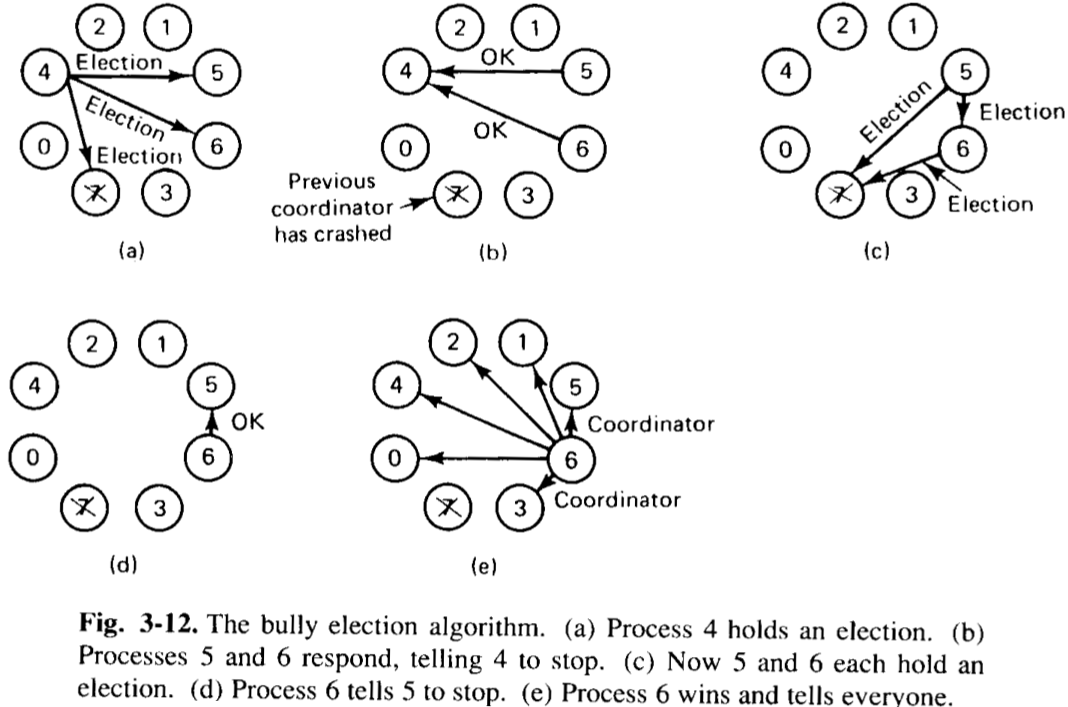
\includegraphics[width=1\textwidth]{Figures/bully_algorithm_drawing.png}
}

% \frame{
% \frametitle{Bully election 5/5}
% \framesubtitle{}
% 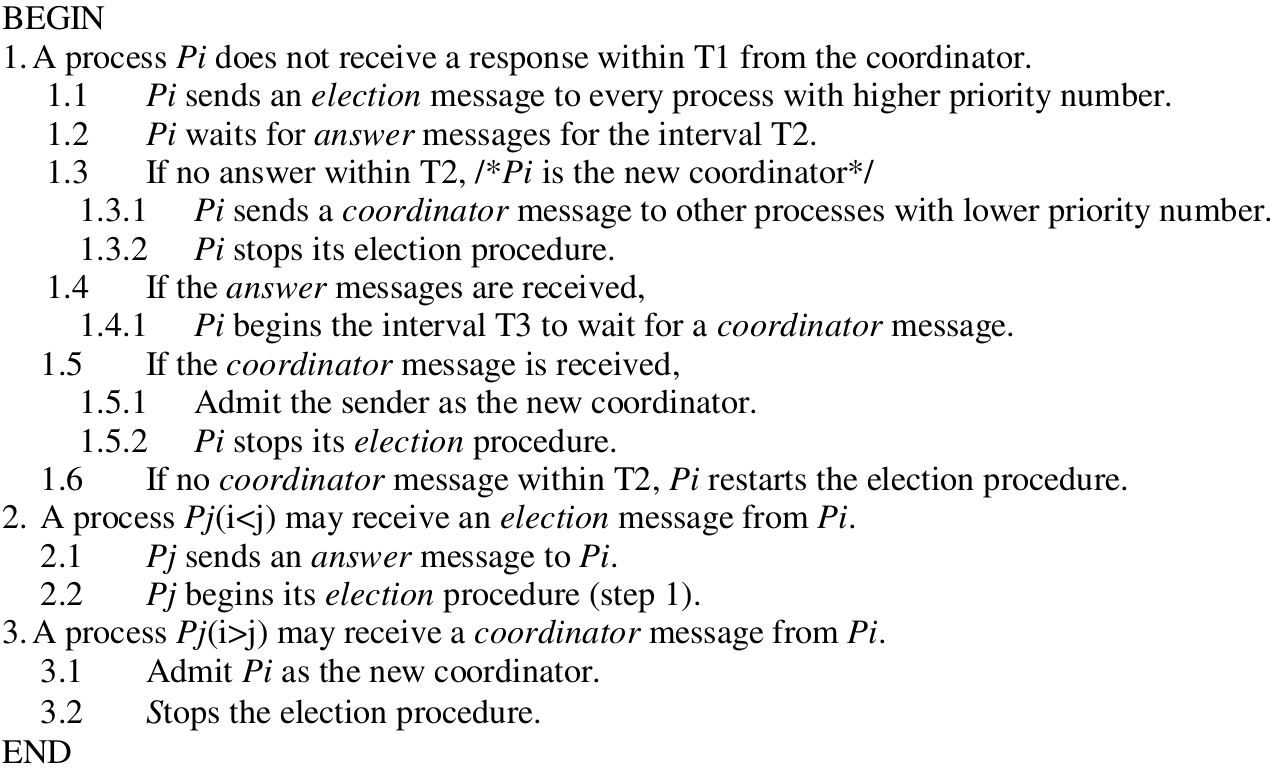
\includegraphics[width=1\textwidth]{Figures/bully_algorithm_listing.png}
% }

\begin{frame}
\frametitle{BE: The algorithm in words}
\framesubtitle{}
Consider processes $\{ P_i \}_{i=0}^{N-1}$ and let id$(P_k) = k$. If
$P_k$ notices a non-responding coordinator, it initiates an election.
\begin{enumerate}
\item $P_k$ sends an \textit{Election} msg to all processes with
  higher IDs%: $P_{k+1}, P_{k+2}, ..., P_{N-1}$
\item $P_k$ awaits \textit{OK} message(s)
  \begin{itemize}
  \item If \textbf{no} msg: $P_k$ becomes leader and sends
    \textit{Coordinator} messages to all processes with lower IDs
  \item If msg: $P_k$ drops out and awaits a \textit{Coordinator} message
  \end{itemize}
\end{enumerate}
\begin{itemize}
\item If a process receives an \textit{Election} message
  \begin{itemize}
  \item Respond w/ \textit{Coordinator} msg if it is the process w/ highest ID
  \item Otherwise, respond w/ \textit{OK} and take over the election
  \end{itemize}
\item If a process receives a \textit{Coordinator} message, it treats  sender as the coordinator
\end{itemize}
\end{frame}


\begin{frame}
\frametitle{BE: Message complexity}
\framesubtitle{}
Assume
\begin{itemize}
\item $N$ processes and \textbf{one} election in progress
\end{itemize}

Best case: Failed process was leader
\begin{itemize}
  \item It sends \textit{Coordinator} msg to all other processes on recovery
  \item Immediate election: $N-1$ messages
\end{itemize}

% \item Second best case
%   \begin{itemize}
%   \item Process with second highest ID notices the coordinator failure
%   \item The process elects itself and sends $n-2$ coordinator messages
%   \end{itemize}

Worst case: Initiator is process with lowest ID, i.e. $P_0$
\begin{itemize}
\item \textit{Election} messages
  \begin{itemize}
  \item $P_0$ sends $N-1$ and $P_1$ sends $N-2$ and ... $\Rightarrow$\\
    $(N-1) + (N-2) + ... + (N - (N-1)) = $\\
    % $\sum_{i=1}^{N-1} N + \sum_{i=1}^{N-1} -i \Rightarrow \mathcal{O}(N^2)$\\
    Left for exercise...
%    $\mathcal{O}((N^2 - N) - k) \Rightarrow \mathcal{O}(N^2)$
  \end{itemize}
\item \textit{OK} messages: Left for exercise...%$\mathcal{O}(N^2)$
\item \textit{Coordinator} messages: Left for exercise...%$\mathcal{O}(N)$
\item Overall message complexity: Left for exercise...%$\mathcal{O}(N^2)$
  % \item Causes $n-2$ processes to begin the election algorithm each sending messages to processes with higher IDs
  % \item Hence the algorithm require $\mathcal{O}(n^2)$ messages
  \end{itemize}
\end{frame}



% \frame{
% \frametitle{The LCR Algorithm: Overview}
% \framesubtitle{}
% \begin{itemize}
% \item LeLann (1977), Chang and Roberts (1979)
% \item Unidirectional
% \item Asynchronous
% \item Non anonymous: every process has an UID
% \item Uniform, i.e. does not depend on \textit{n}
% \item Comparison-based Algorithm
% \item The size of the ring is unknown to the processes
% \item Unidirectional Ring
% \item It elects the process with the maximum UID
% \end{itemize}
% }

% \frame{
% \frametitle{The LCR algorithm: Description}
% \framesubtitle{}
% Each process sends its UID around the ring. When a process receives a
% UID, it compares this one to its own.
% \begin{itemize}
% \item If the incoming UID is greater, then it passes this UID to the
%   next process.
% \item If the incoming UID is smaller, then it discards it.
% \item If it is equal, then the process declares itself the leader.
% \end{itemize}
% }


% \frame{
% \frametitle{The LCR Algorithm: Correctness}
% \framesubtitle{}
% \begin{itemize}
% \item Messages from process with highest ID are never discarded
% \item Thus, the \textbf{corrrect} leader is elected
% \item No other process UID can traverse the entire ring
% \item Thus, no other UID is elected 
% \end{itemize}
% }

\section[LCR]{LeLann-Chang-Roberts}

\frame{
\frametitle{LCR: Background}
\framesubtitle{}
Proposed by
\begin{itemize}
\item E. G. Chang and R. Robert, "An improved algorithm for decentralized extreme-finding in
circular configurations of processors," Communications of ACM, vol. 22, no. 9, pp. 281-283, 1979
\item Note: The explanation in the course book by Marten van Steen is
  not fully equivalent with the explanation given in the paper by
  Chang and Robert. We will adhere to the book.
\end{itemize}
Leader election process begins
\begin{itemize}
\item Leader halts processing
\item If a process that was previously down comes back up, it holds an election.
\end{itemize}
End result
\begin{itemize}
\item One and \textbf{only one} leader
\item Process with highest ID elected leader
\end{itemize}
}


\begin{frame}
  \frametitle{LCR: Assumptions}
  \begin{itemize}
  \item Processes are arranged in a logical unidirectional ring
  \item All processes knows the structure of the ring
  \item Each process has a unique ID
  \item Processes know each other's process ID
  \item Processes do not know which ones are currently alive
  \item Each process can compare IDs (e.g. to find the highest)
  \item All processes can communicate with clockwise neighbor
  \item A failed process is always detectable
  \item Any process can initiate an election
  \item Upon failure recovery, the process knows it failed
  \end{itemize}
\end{frame}


\begin{frame}
  \frametitle{LCR: Message types}
  \begin{itemize}
  \item \textit{Election}: Message to announce election
  \item \textit{Coordinator}: Message to announce ID of new coordinator
  \end{itemize}

\end{frame}


\frame{
\frametitle{LCR: The algorithm illustrated}
\framesubtitle{}
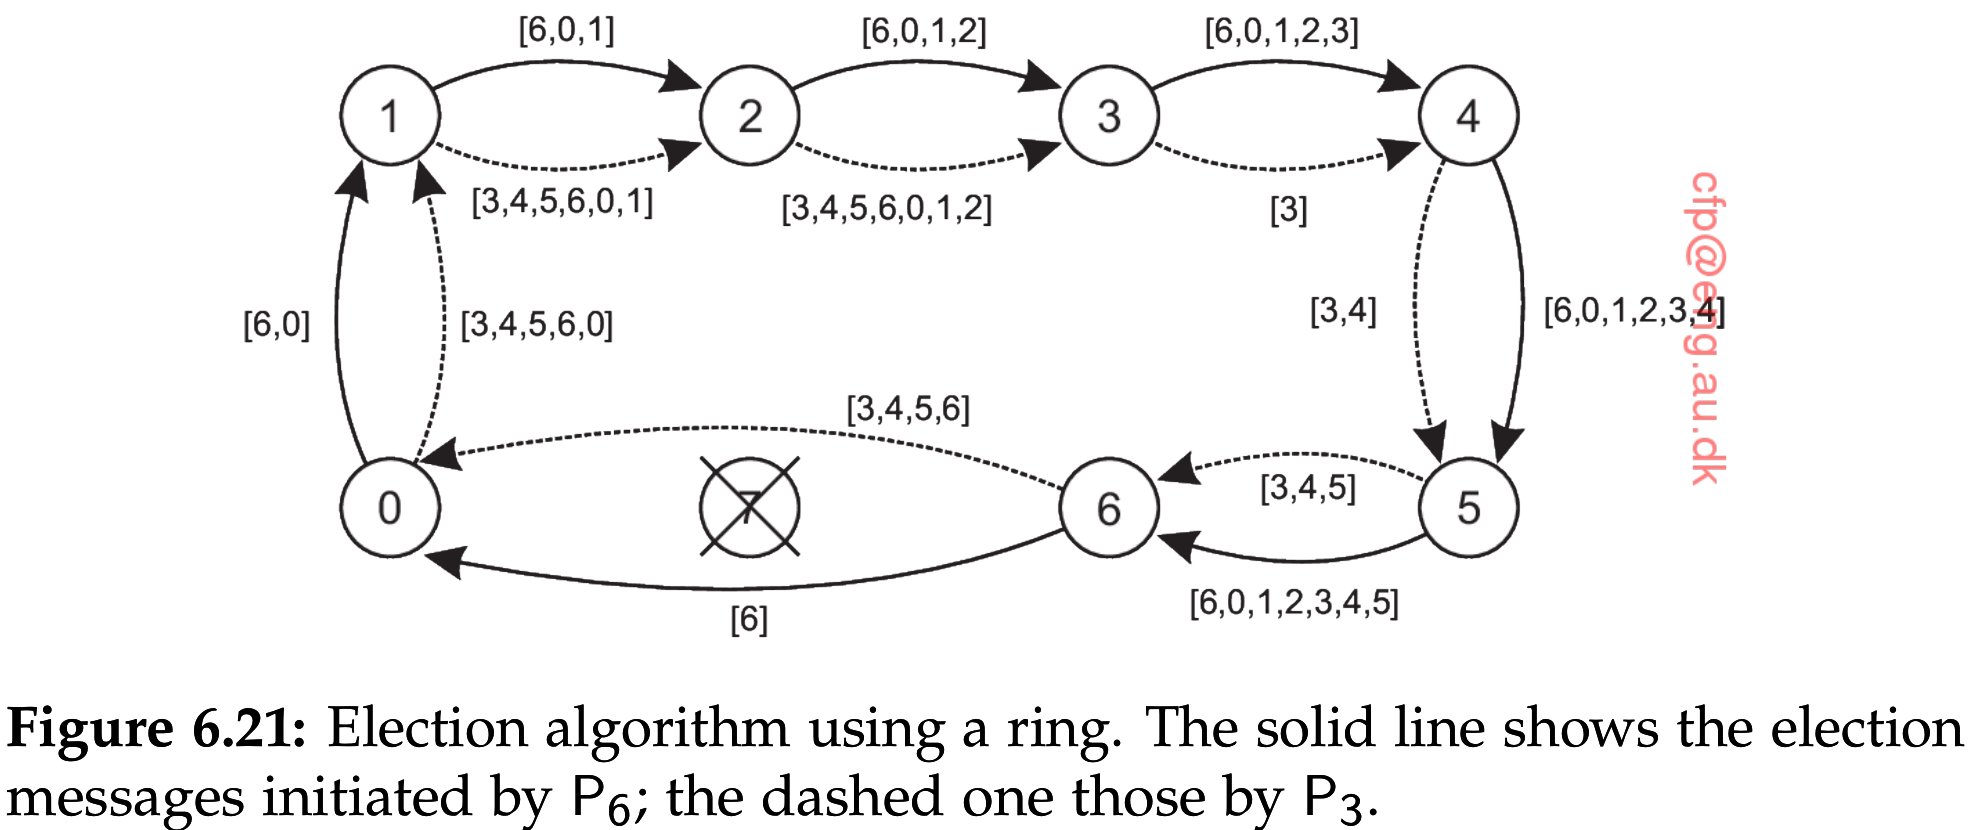
\includegraphics[width=1\textwidth]{Figures/ring_election.png}
}


\frame{
\frametitle{LCR: The algorithm in words}
\framesubtitle{}
\begin{itemize}
\item A process initiates an election if
  \begin{itemize}
  \item it just recovered from failure or
  \item if it notices that the leader has failed
  \end{itemize}
\item Initiator sends \textit{Election} msg to closest live clockwise neighbor
\begin{itemize}
\item Election message is forwarded around the ring
\item Each process adds its own ID to the \textit{Election} message
\end{itemize}
\item When \textit{Election} message returns
  \begin{itemize}
  \item Initiator picks node with highest ID
  \item Sends a \textit{Coordinator} message specifying the election winner
  \item Also, IDs with all living members are attached in order to update all members of this
  \end{itemize}
\begin{itemize}
\item Coordinator message is removed when it has circulated once
\end{itemize}
\item Multiple elections can be in progress simultaneously
\end{itemize}
}

\frame{
\frametitle{LCR: Message complexity}
\framesubtitle{}
Assume
\begin{itemize}
\item \textit{N} processes and \textbf{one} election in progress
\end{itemize}

Best case = Worst case
  \begin{itemize}
  \item Always $2N$ messages, i.e. $\mathcal{O}(N)$
  \item One round for the election message
  \item One round for the coordinator message
  \end{itemize}
}

\section[MAH]{Election in mobile ad hoc (MAH) networks}

\frame{
\frametitle{MAH: Background}
\framesubtitle{}
Proposed by
\begin{itemize}
\item Vasudevan S., Kurose J.F. and Towsley D.F., ``Design and
  Analysis of a Leader Election Algorithm for Mobile Ad Hoc
  Networks''. In 12th International Conference on Network Protocols,
  pp. 350–360, Los Alamitos, CA., Oct. 2004. IEEE Computer Society
  Press.
\end{itemize}
Properties
\begin{itemize}
\item For wireless/mobile ad hoc networks
\item Handles failing nodes and network partitions
\end{itemize}
End result
\begin{itemize}
\item The best (wrt. \textbf{resources}) leader elected
\end{itemize}
}


\begin{frame}
  \frametitle{MAH: Assumptions}
  \begin{itemize}
  \item Each process has a unique ID
  \item Processes know each other’s process ID
  \item Processes do not know which ones are currently alive
  \item Each process can compare IDs (e.g. to find the highest)
  \item All processes can inter-communicate
  \item A failed process is always detectable
  \item Any process can initiate an election
  \item Upon failure recovery, the process knows it failed
  \item The course book disregards that
    \begin{itemize}
    \item nodes can move physically, i.e. topology is not static
    \item message passing is unreliable particularly in wireless net
    \end{itemize}
  \end{itemize}
\end{frame}


\frame{
\frametitle{MAH: Message types}
\framesubtitle{}
\begin{itemize}
\item \textit{Election}: Message to announce election
  \begin{itemize}
  \item To neighbors within range
  \item \textit{Election-ID}: Each election process is tagged with an
    unique ID. When multiple elections are initiated, each node will
    decide to join only one election, i.e. the one with the highest ID
    (stopping any running participation in other elections.)
  \end{itemize}
\item \textit{Acknowledgement}: Msg in response to election msg
  \begin{itemize}
  \item Acknowledge the receipt of \textit{Election} msg. 
  \end{itemize}
%\item \textit{Coordinator}: Message to announce ID of new coordinator
\end{itemize}
}


\frame{
\frametitle{MAH: The algorithm illustrated}
\framesubtitle{}
\begin{figure}[htbp!]
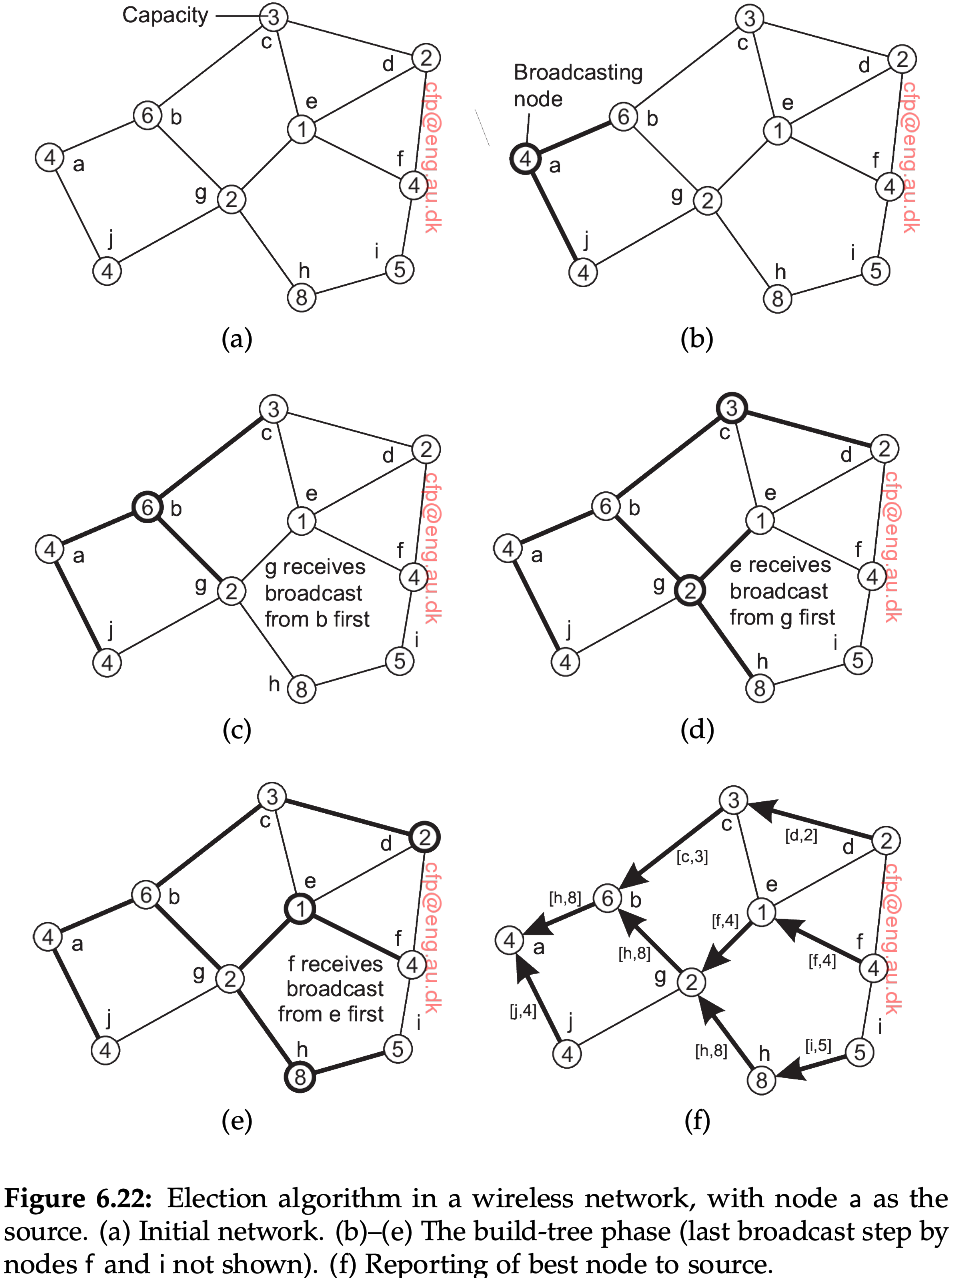
\includegraphics[width=0.52\textwidth]{Figures/wireless_adhoc_election.png}
%\caption{Caption here...}
%\label{fig:}
\end{figure}
}

\begin{frame}
  \frametitle{MAH: The algorithm in words}
  \begin{itemize}
  \item Any node can initiate an election by broadcasting \textit{Election} msg
  \item Nodes within range receive the \textit{Election} msg
  \item When a node receives an \textit{Election} msg for the first
    time
    \begin{enumerate}
    \item it designates the sender as its \textit{parent}
    \item sends out \textit{Election} msg to nodes within range (except parent)
    \item waits for ack's to return before ack'ing \textit{Election}
      from parent.\\ The \textit{Acknowledgement} \textbf{also}
      contain a resource status.\\ The resource status reported back
      is of the \textbf{best} (by some metric and comparison) of the
      incoming
      statuses.\\
    \end{enumerate}
  \item When a node receives an \textit{Election} msg from a
    non-parent node, it merely acknowledges the receipt.\\ The
    \textit{Acknowledgement} \textbf{does not} contain a resource status
  \end{itemize}
\end{frame}

\section[HS]{Hirschberg-Sinclair}

\frame{
\frametitle{HS: Background}
\framesubtitle{}
Proposed by
\begin{itemize}
\item D.S. Hirschberg and J.B. Sinclair, ``Decentralized
  extrema-finding in circular configurations of processors'',
  Communications of the ACM, 23 (11), 1980
\end{itemize}
Leader election process begins
  \begin{itemize}
  \item Leader halts processing
  \item If a process that was previously down comes back up, it holds
an election.
  \end{itemize}
  End result
  \begin{itemize}
  \item One and \textbf{only one} coordinator
  \item Leader (highest ID) election in bidirectional rings
  \item Message complexity $\mathcal{O}_m = (n \log n)$ 
  \end{itemize}
}

\begin{frame}
  \frametitle{HS: Assumptions}
  \begin{itemize}
  \item Each process has a unique ID 
  \item Processes do not know each other’s process ID
  \item The process with highest ID is elected
  \item Ring size (no. of processes) initially unknown to the processes
  \item Communication is asynchronous
  \end{itemize}

\end{frame}

\frame{
\frametitle{HS: Message types}
\begin{itemize}
\item \texttt{SendBoth}: Send messages in both directions
\item \texttt{SendPass}: Pass received message on
\item \texttt{SendEcho}: Send response message back
\end{itemize}
}



\frame{
\frametitle{HS: Neighbourhood elections}
\framesubtitle{}
Elections are performed in neighbourhoods
\begin{itemize}
\item The \textbf{$2^k$-neighbourhood} of a process $p$ is the \textbf{set of
  processes} that are at distance at most $2^k$ from $p$ ($2^k$
  left-neighbours plus $2^k$ right-neighbours)
\item Phases $k = 0, 1, 2, ...$
\item For each $k$, process $i$ sends its ID through $2^k$ bidirectionally
\item If both ID tokens return, then $i$ continues to phase $k+1$
\end{itemize}
\begin{figure}[htbp!]
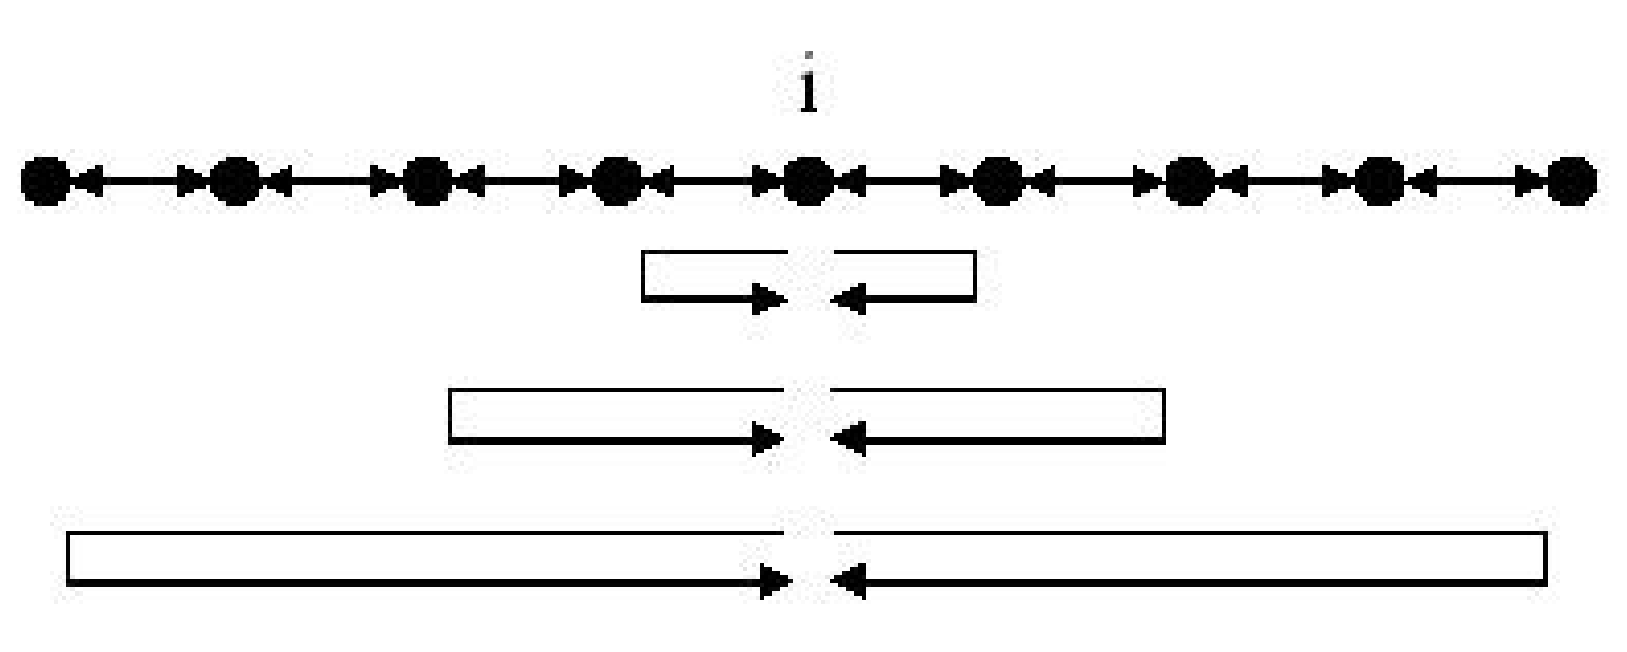
\includegraphics[width=0.7\textwidth]{Figures/hs_neighbourhood.png}
\caption{Execution of HS (by courtesy of Mitsou Valia)}
\label{fig:}
\end{figure}
}

\frame{
\frametitle{HS algorithm: Election phases}
\framesubtitle{}  
Elections are carried out in (asynchronous) phases
\begin{itemize}
\item Phases $k = 0, 1, 2, ...$
\item Process $p_i$ tries to become a leader in phase $k$ in its $2^k$-neighbourhood
\item Only if $p_i$ is the winner, i.e. it has the
  highest ID in its $2^k$-neighbourhood, it can proceed to phase
  $k+1$
\item In each phase, the process $p_i$ sends out tokens containing $ID_i$ in both directions
\item Tokens travel distance $2^k$ and return to $p_i$
\item The size of the neighbourhood doubles in each phase (i.e. $2^k$)
\item Fewer $p$'s proceed to higher phases, until a single winner gets elected in the whole ring.
\end{itemize}
}

\frame{
\frametitle{HS algorithm: Sending messages 1/2}
\framesubtitle{}
\begin{itemize}
\item Initially, all $p$'s initiate a candidancy (phase 0), e.g. after having
received a broadcasted request for electing a leader
\item The \textbf{election-messages} sent by candidates contain 3 fields:
  \begin{itemize}
  \item The ID of the candidate.
  \item The current phase number $k$
  \item A hop counter $d$, which is initially 0 and is incremented by
    1 whenever the message is forwarded to the next process $p$
  \end{itemize}
\item If a $p_j$ receives a msg with \texttt{(r, k, d)} where
  $d = 2^k$, then it is the last process in the $2^k$ -neighbourhood
  of $p_r$ with ID $= r$
\end{itemize}
}

\frame{
\frametitle{HS algorithm: Sending messages 2/2}
\framesubtitle{}
\begin{itemize}
\item If the $p_i$ receiving the election message has a greater ID, then it
swallows the message, otherwise it relays it to the same direction,
after incrementing $d$ by 1.
\item If the message makes it till the $2^k$-distance $p_i$, then $p_i$ sends back
a \textbf{reply-message}, which is forwarded till it reaches the candidate $p_r$
\item If the candidate receives replies from both directions, then it is the
winner of its $2^k$-neigbourhood
\item A $p_i$ that receives an election message with its own ID is the
  leader of the ring.
\item The leader should also announce itself to all other nodes
\end{itemize}
}

\frame{
\frametitle{HS algorithm: Correctness}
\framesubtitle{}
\begin{itemize}
\item Messages from process with highest ID are never discarded
\item Thus, the correct leader is elected
\item No other process ID can traverse the entire ring
\item Therefore, no one else is elected 
\end{itemize}
}

% \frame{
% \frametitle{The HS algorithm: Execution / graphical}
% \framesubtitle{}
% \begin{figure}[htbp!]
% 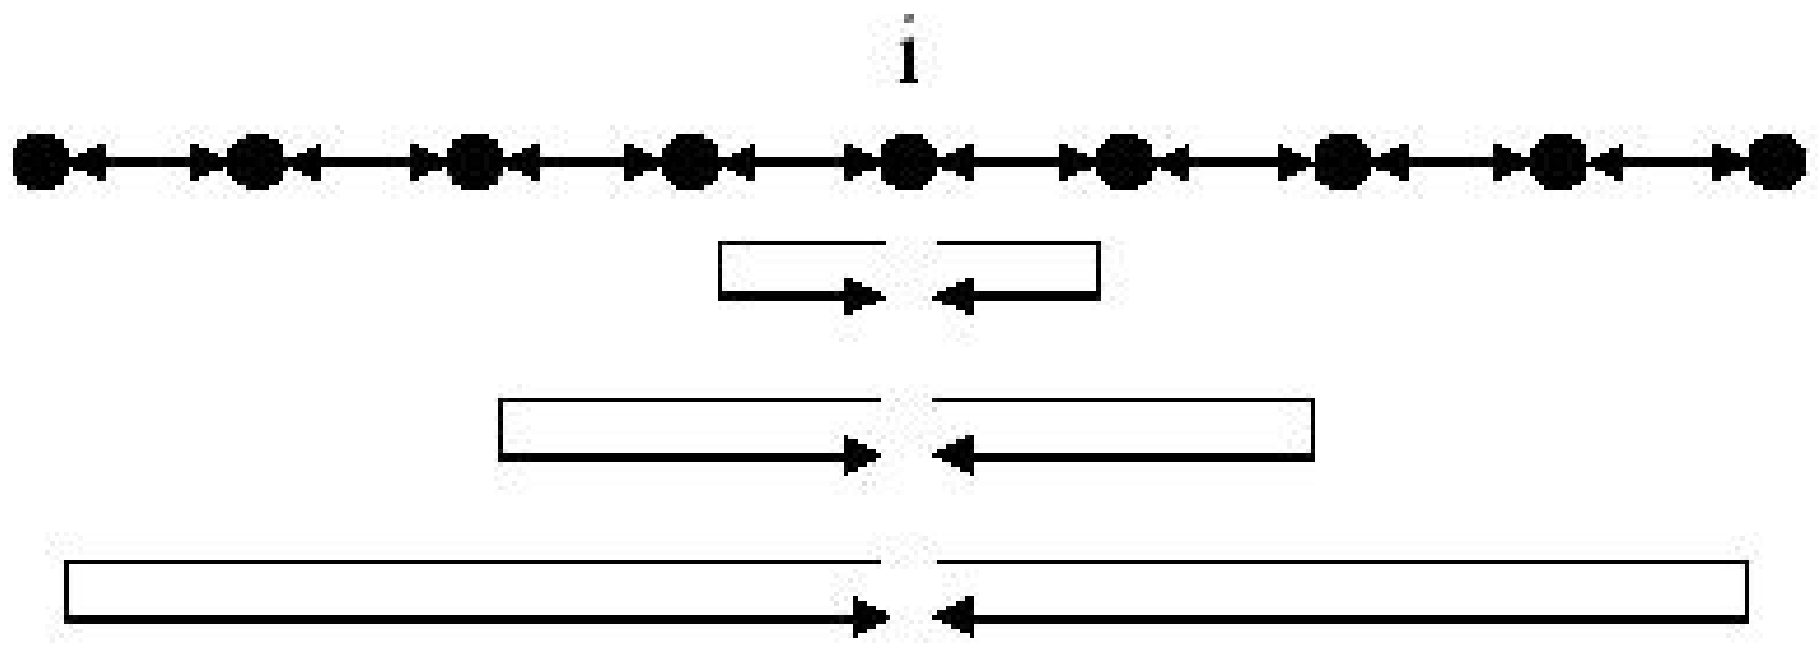
\includegraphics[width=0.7\textwidth]{Figures/hs_leader_elect.png}
% \caption{Fig. by courtesy of Mitsou Valia}
% \label{fig:}
% \end{figure}
% }

% \frame{
% \frametitle{The HS algorithm: Execution / description}
% \framesubtitle{}
% When a process receives an outgoing UID, it
% compares this one with its own.
% \begin{itemize}
% \item If the received UID is smaller, then it discards it.
% \item If the received UID is greater then
%   \begin{itemize}
%   \item it passes it to the next process, if it is not the end of its path,
%   \item else it returns it back to the previous one (to travel back to the originating process).
%   \end{itemize}
% \item If it is equal, then the process declares
% itself the leader.
% \end{itemize}
% }

\frame{
\frametitle{HS algorithm: Example (phase 0)}
\framesubtitle{}
\begin{figure}[htbp!]
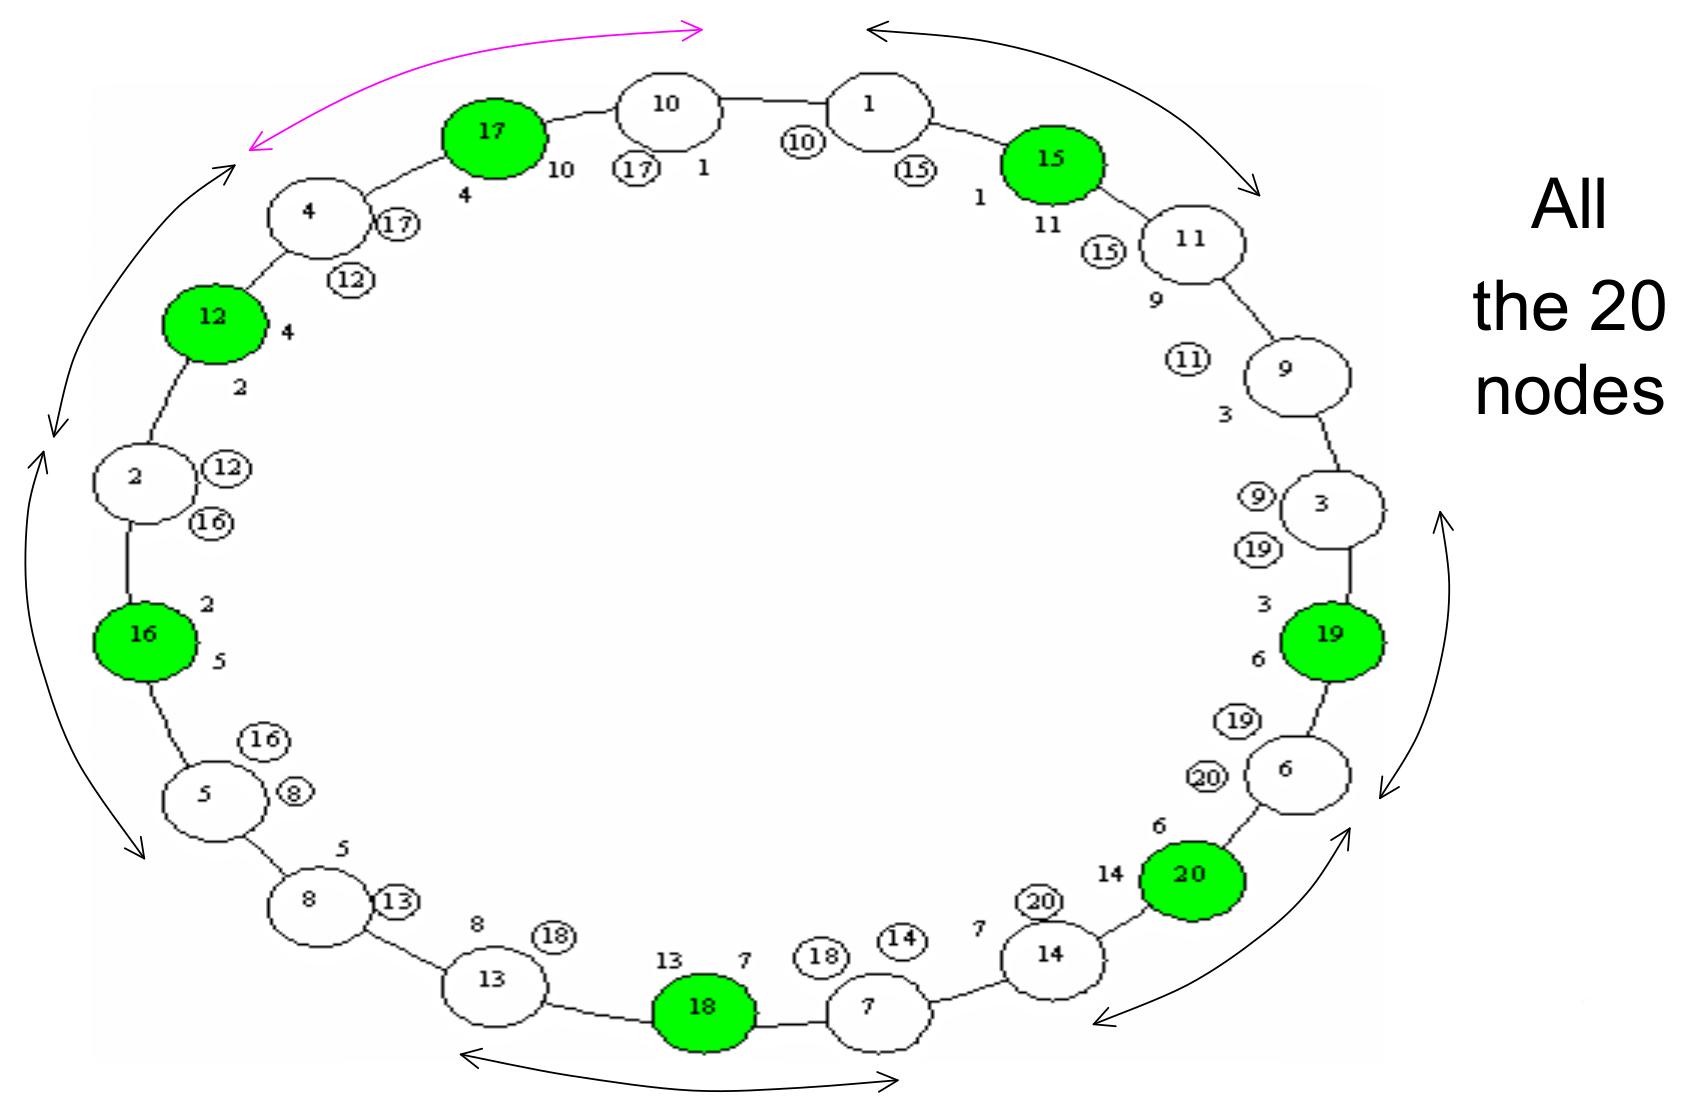
\includegraphics[width=0.7\textwidth]{Figures/hs_phase0.png}
\caption{Fig. by courtesy of Mitsou Valia}
\label{fig:}
\end{figure}
}

\frame{
\frametitle{HS algorithm: Example (phase 1)}
\framesubtitle{}
\begin{figure}[htbp!]
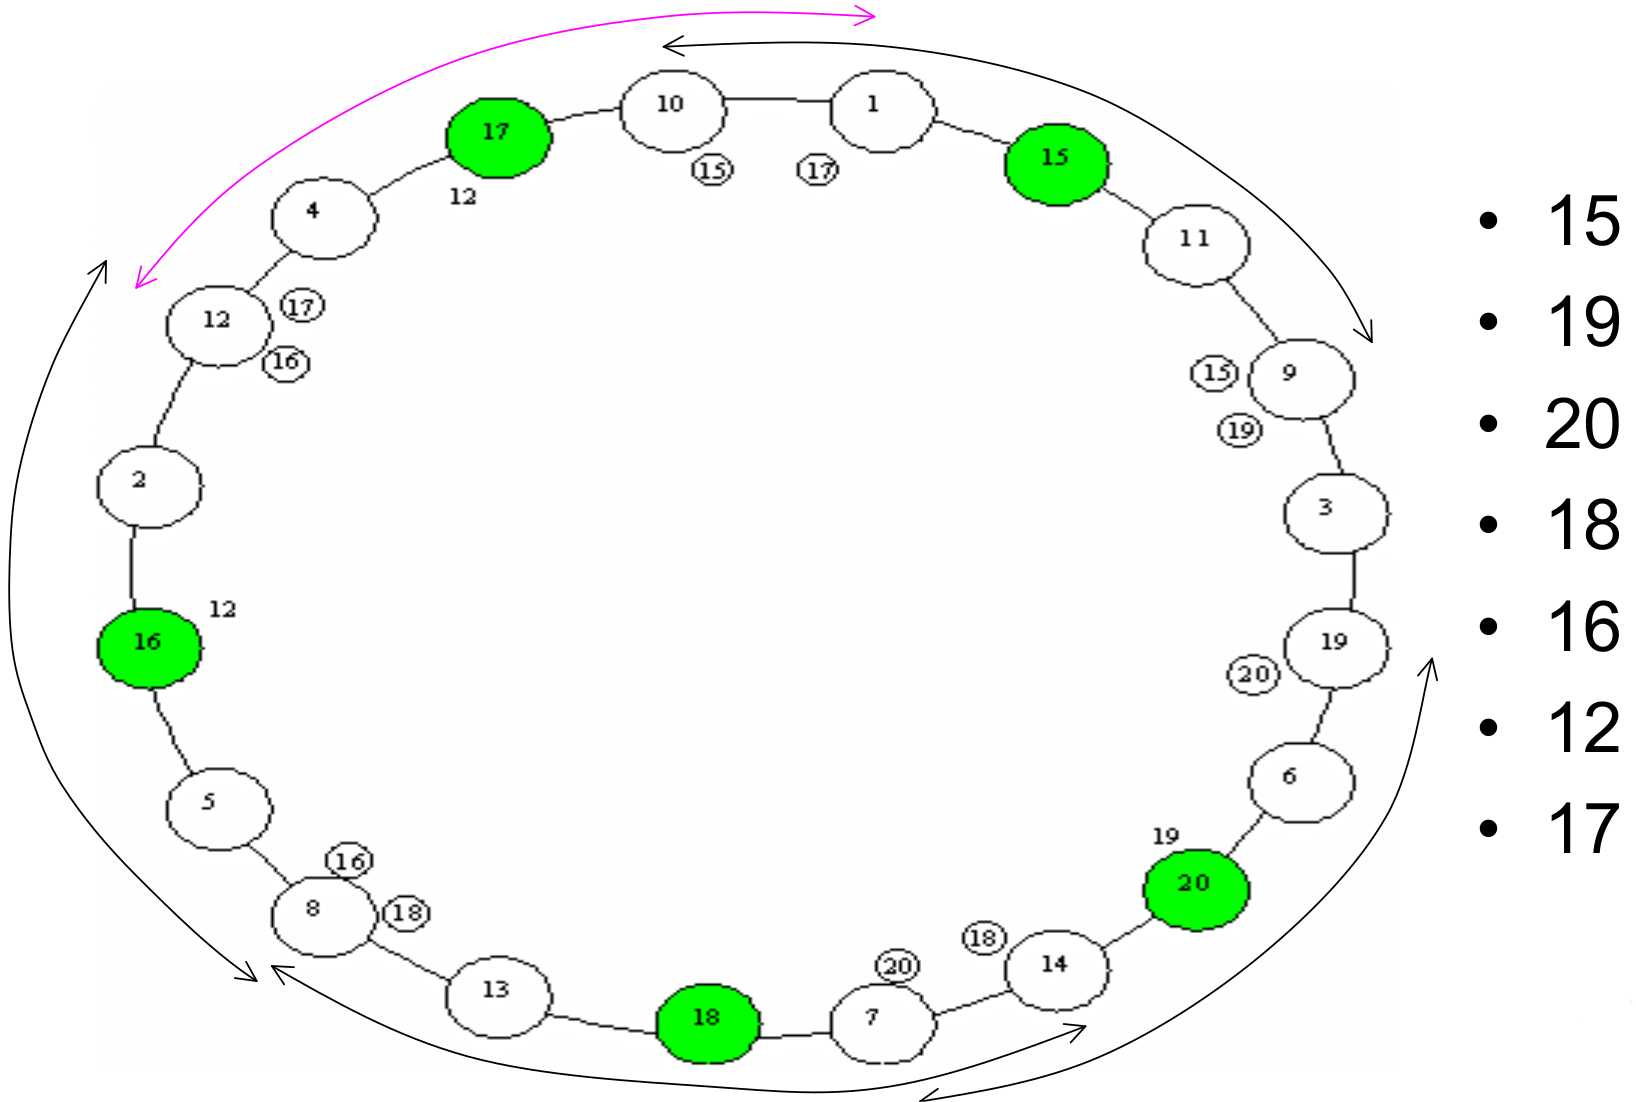
\includegraphics[width=0.7\textwidth]{Figures/hs_phase1.png}
\caption{Fig. by courtesy of Mitsou Valia}
\label{fig:}
\end{figure}
}

\frame{
\frametitle{HS algorithm: Example (phase 2)}
\framesubtitle{}
\begin{figure}[htbp!]
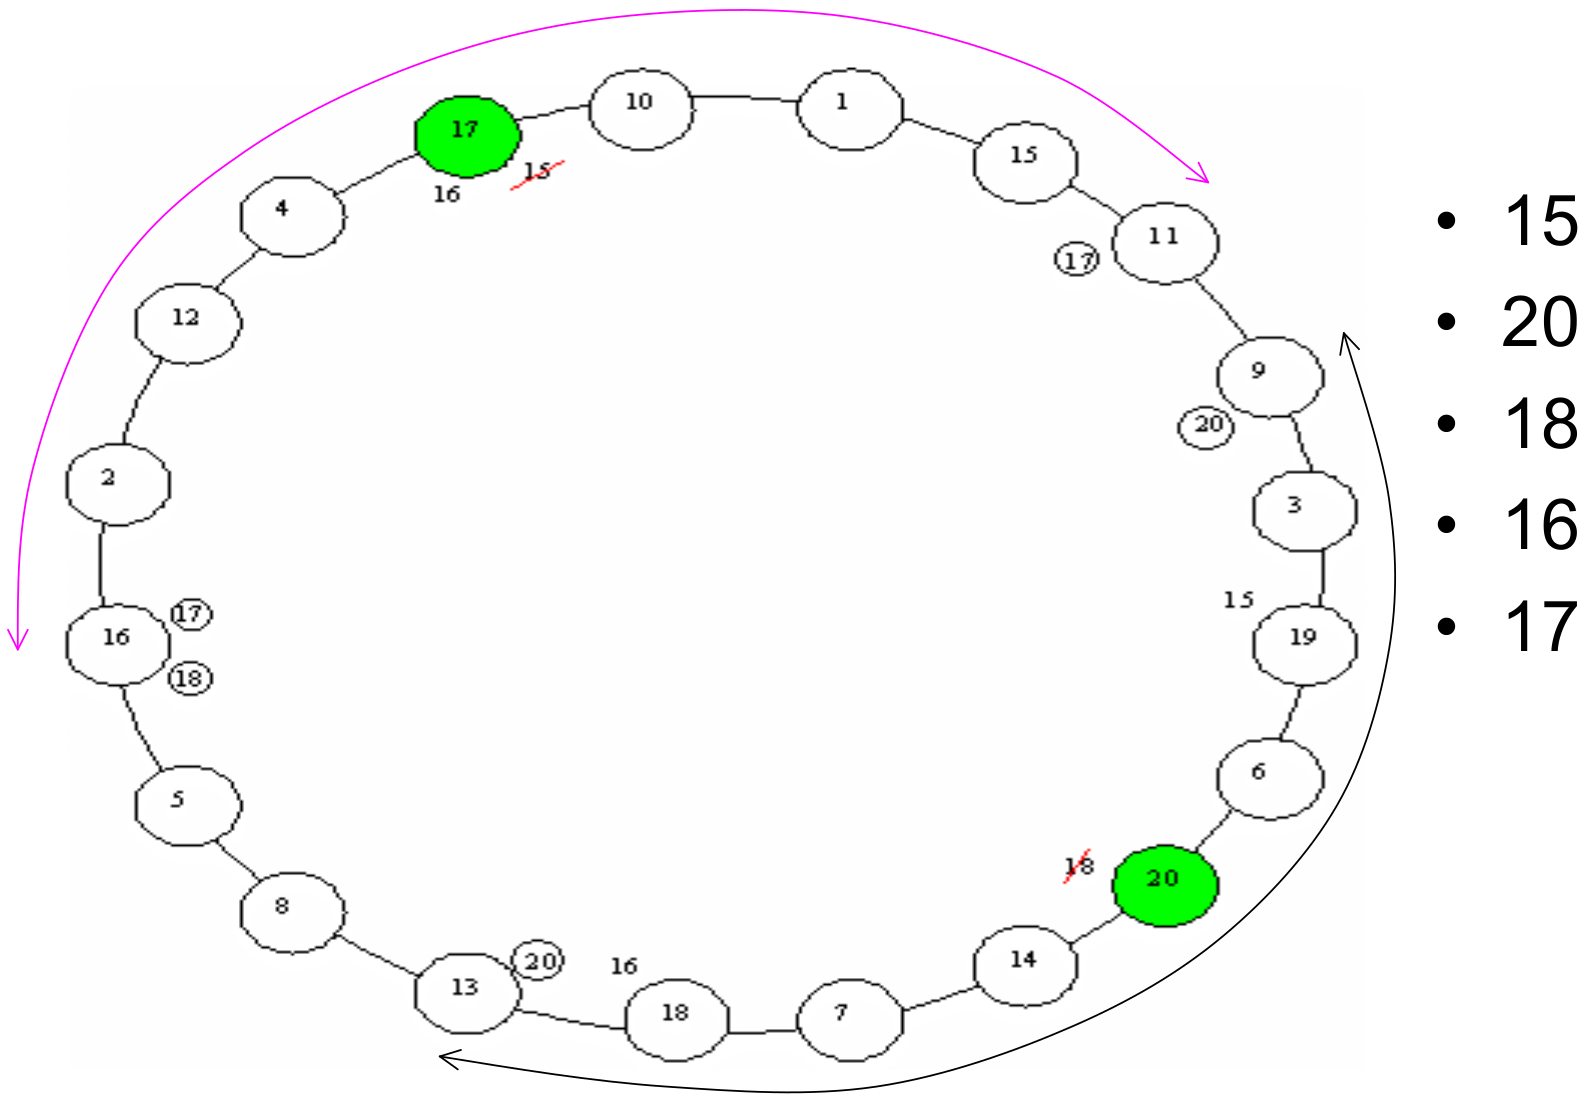
\includegraphics[width=0.7\textwidth]{Figures/hs_phase2.png}
\caption{Fig. by courtesy of Mitsou Valia}
\label{fig:}
\end{figure}
}

\frame{
\frametitle{HS algorithm: Example (phase 3)}
\framesubtitle{}
\begin{figure}[htbp!]
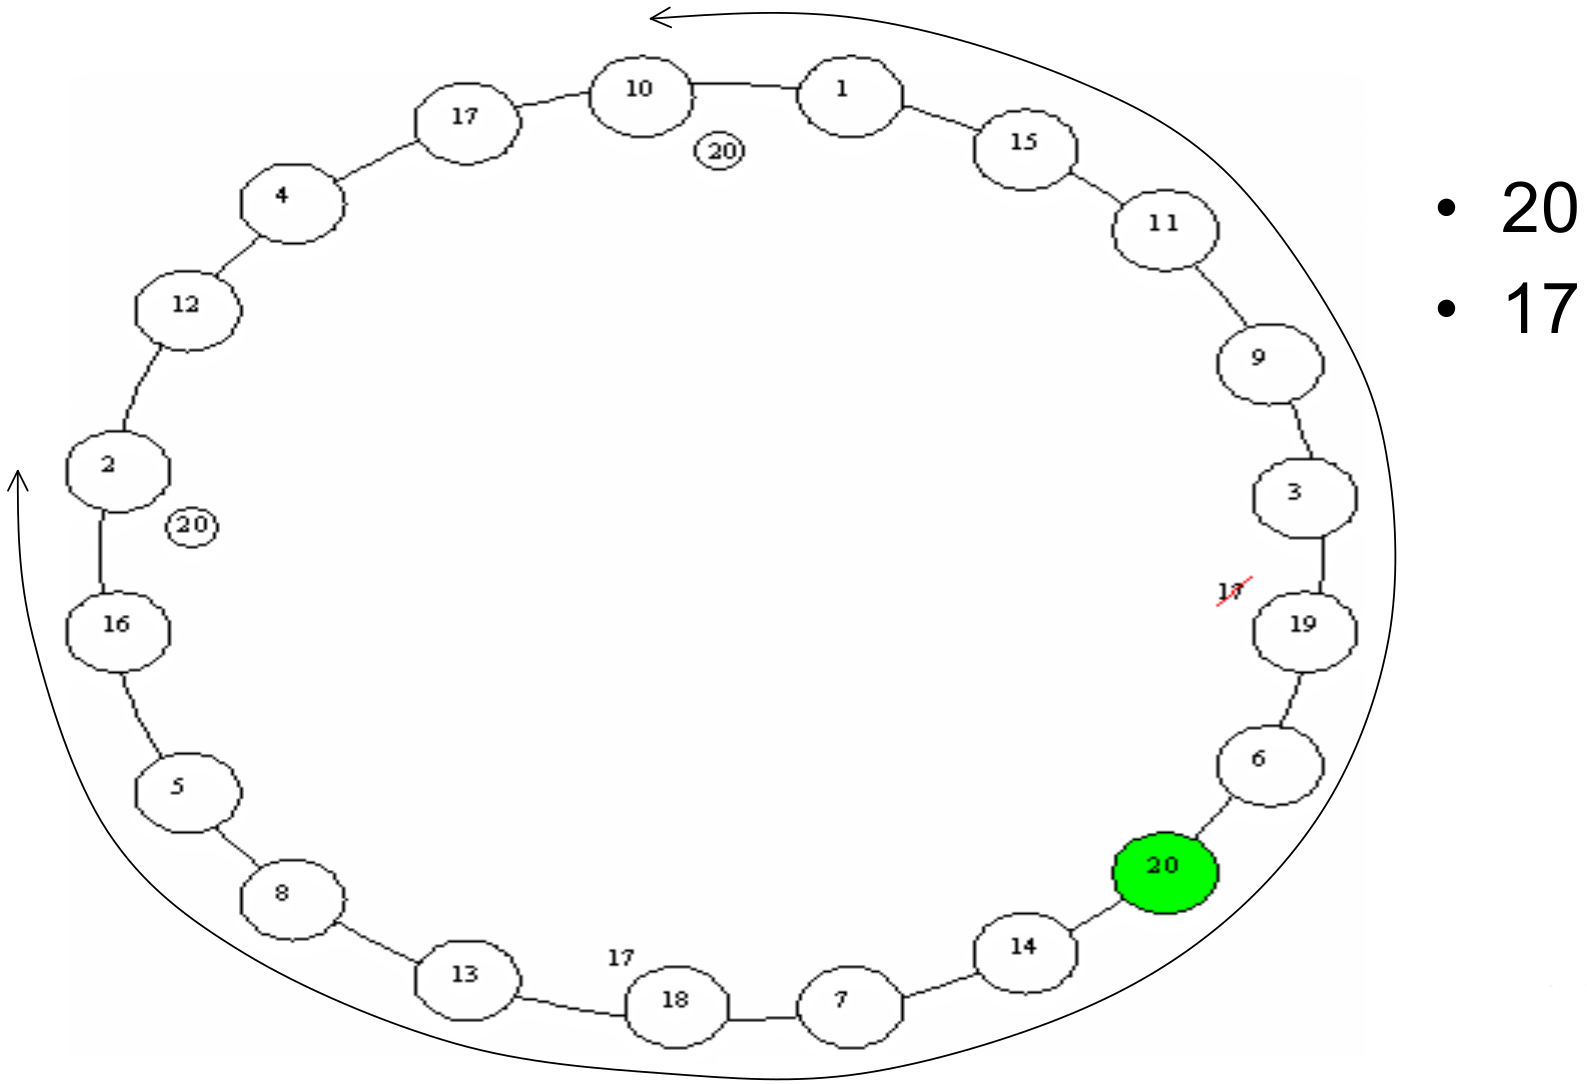
\includegraphics[width=0.7\textwidth]{Figures/hs_phase3.png}
\caption{Fig. by courtesy of Mitsou Valia}
\label{fig:}
\end{figure}
}

\frame{
\frametitle{HS algorithm: Example (phase 4)}
\framesubtitle{}
\begin{figure}[htbp!]
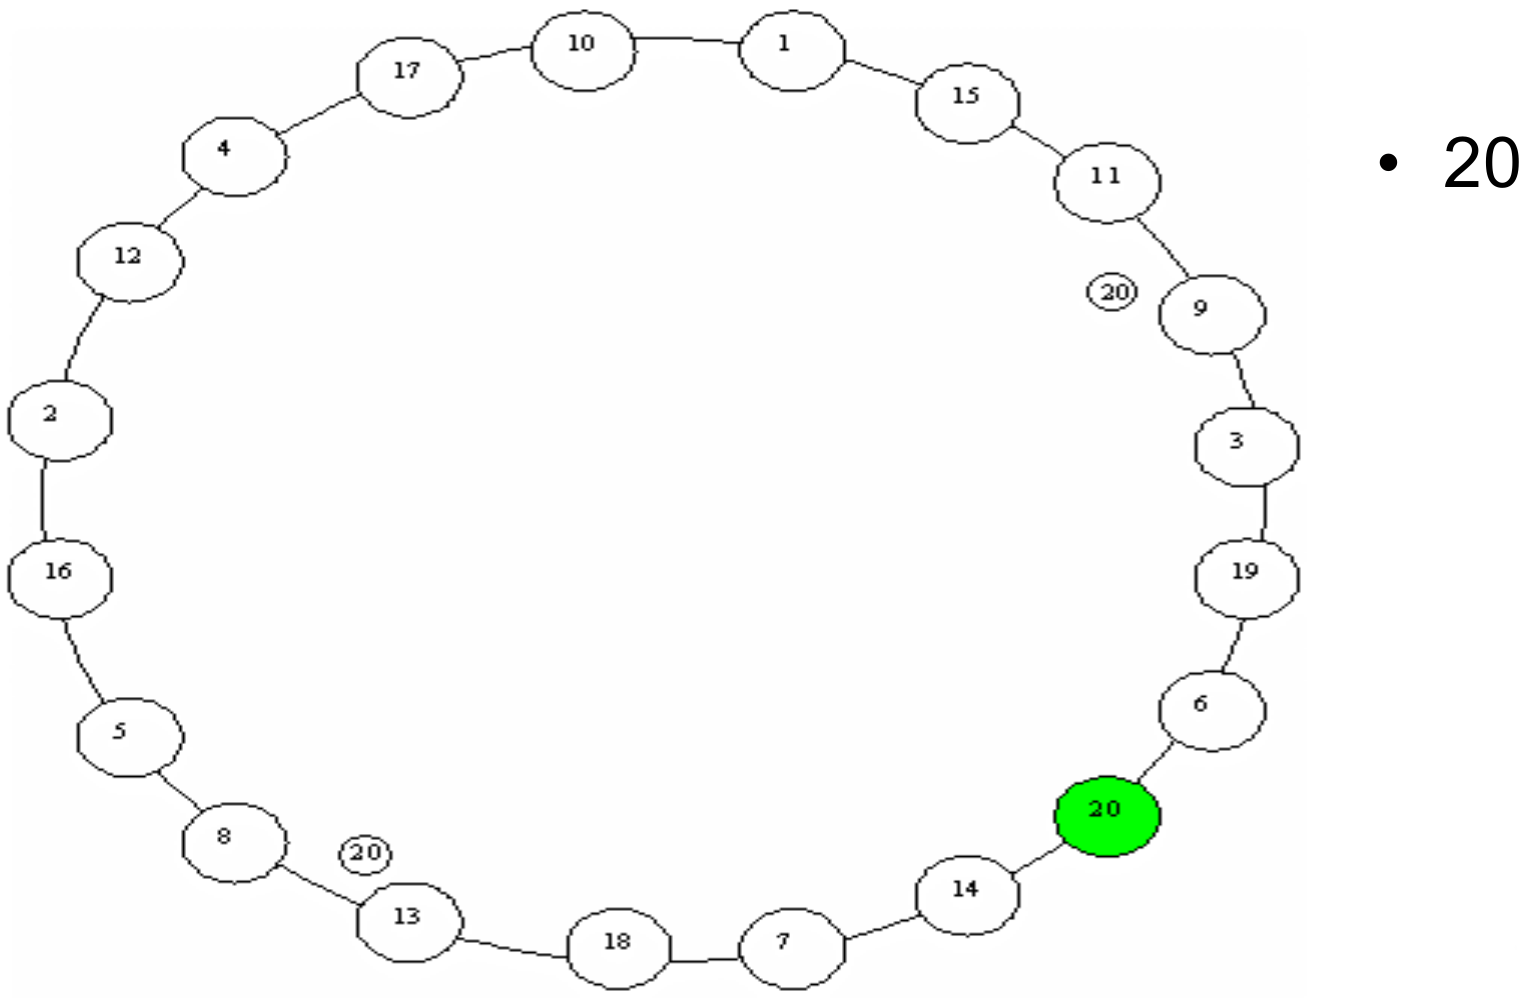
\includegraphics[width=0.7\textwidth]{Figures/hs_phase4.png}
\caption{Fig. by courtesy of Mitsou Valia}
\label{fig:}
\end{figure}
}

\frame{
\frametitle{HS algorithm: Example (phase 5)}
\framesubtitle{}
\begin{figure}[htbp!]
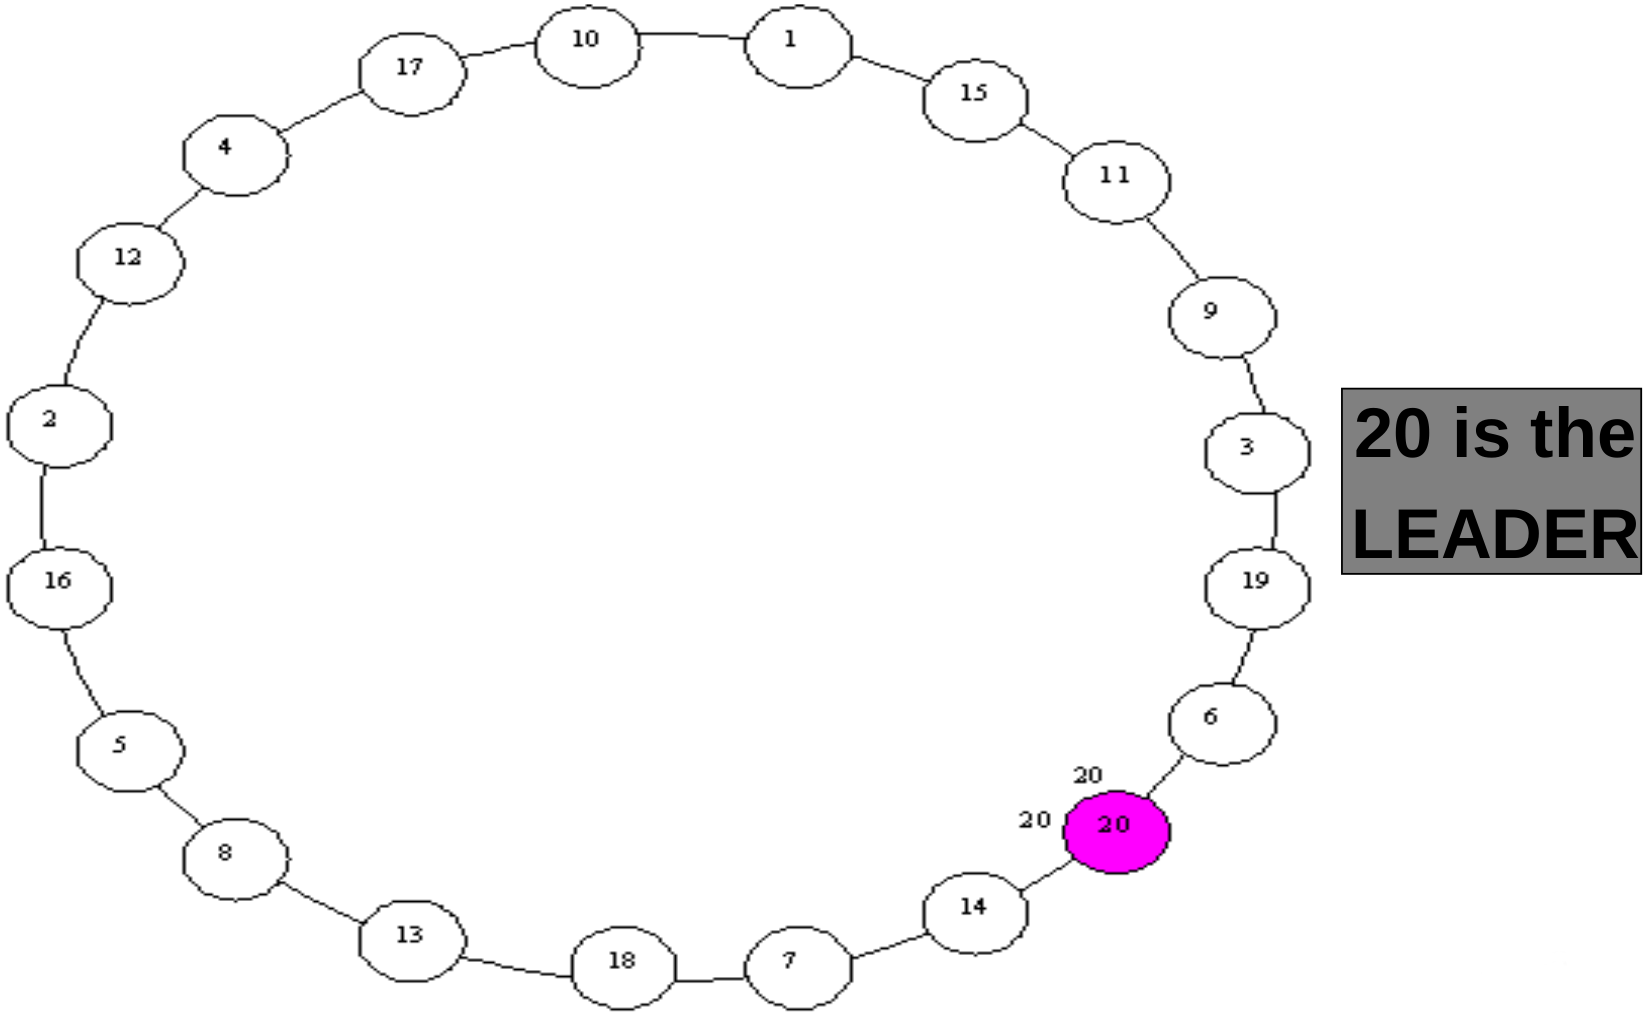
\includegraphics[width=0.7\textwidth]{Figures/hs_phase5.png}
\caption{Fig. by courtesy of Mitsou Valia}
\label{fig:}
\end{figure}
}






%\section[LCR]{LeLann-Chang-Roberts}
%\section[HS]{Hirschberg-Sinclair}
%\section[Peterson]{Peterson}


%\section[References]{References}
% %===============References
% \begin{frame}[allowframebreaks]
% \frametitle{References}
% %\def\section*#1{}%remove auto heading for references
% \fontsize{5pt}{5pt}\selectfont
% \def\newblock{\hskip .11em plus .33em minus .07em}
% \bibliographystyle{chicago}
% \bibliography{/home/cfp/SyncAU/Library/MyLatex/cfp_bibliography}
% \normalsize
% \end{frame}

\end{document}

% \begin{figure}
% \includegraphics[width=0.7\textwidth]{Figures/filename.pdf}
% \caption{Caption here...}
% \end{figure}

% c:=vertical centered. t:= top vertically aligned. T:=alt. top-align better for graphics
% \begin{columns}[t] 
% \begin{column}[T]{0.46\textwidth}
% \end{column}
% \begin{column}[T]{0.46\textwidth}
% \end{column}
% \end{columns}

% \begin{table}[htbp]
% \begin{tabular}[c]{>{\raggedright}p{0.25\linewidth}|>{\raggedright\arraybackslash}p{0.65\linewidth}}
% \toprule
% \textbf{abc} & \textbf{def}\\
% \midrule\midrule
% ... & ...\\\hline
% ... & ...\\
% \bottomrule
% \end{tabular}
% \end{table}
% }